\documentclass{sig-alternate}
\usepackage[numbers, sort, compress]{natbib}
\usepackage{graphics}
\usepackage{graphicx}
\usepackage{epstopdf}
\usepackage{color}
\usepackage{hyperref}
\usepackage{pdfsync}
\usepackage{mdwlist}


\begin{document}

\conferenceinfo{TeraGrid 11} {}
\CopyrightYear{2011}
\crdata{}
%\clubpenalty=10000
%\widowpenalty = 10000


\title{Building Gateways for Life-Science Applications using the
  Distributed Adaptive Runtime Environment (DARE) Framework}

\numberofauthors{3}
\author{
\alignauthor Joohyun Kim\\
       \affaddr{Center for Computation and Technology}\\
       \affaddr{Louisiana State University}\\
       \affaddr{216 Johnston}\\
       \affaddr{Baton Rouge, LA} \\
       \email{jhkim@cct.lsu.edu}
\alignauthor Sharath Maddineni\\
       \affaddr{Center for Computation and Technology}\\
       \affaddr{Louisiana State University}\\
       \affaddr{216 Johnston}\\
       \affaddr{Baton Rouge, LA}
       \email{smaddineni@cct.lsu.edu}
\alignauthor Shantenu Jha\titlenote{Author for correspondence}\\
      \affaddr{Center for Computation and Technology}\\
     \affaddr{Louisiana State University}\\
      \affaddr{214 Johnston}\\
      \affaddr{Baton Rouge, LA}
     \email{sjha@cct.lsu.edu}
}

\maketitle


\begin{abstract}
  We introduce the Distributed Adaptive Runtime Environment (DARE)
  framework that is a SAGA-based higher-level abstraction, and
  demonstrate its effectiveness as an integral component of a
  wide-range of life-science gateways.  An understanding of challenges
  and computational requirements of the life-science applications in
  distributed heterogeneous scalable HPC resources has led to the
  development of the DARE framework with which a lightweight,
  extensible, versatile gateway that seamlessly utilizes scalable
  infrastructure can be built for a life-science application
  effectively.  DARE science gateways comprise a user access layer and middleware layers
  built upon Simple API for Grid Application (SAGA) and the SAGA-based
  Pilot-Job (SAGA-BigJob) capability.  This work is predicated on
  three important trends: (i) that the importance, impact and percentage of
  TeraGrid/XD resources assigned to the life sciences is increasing at
  a rate that is probably greater than other disciplines, (ii) that
  gateways have proven to be a very effective access mechanism to
  distributed HPC resources provided by the TG/XD, and in particular a
  very successfull model for shared/community access models, and (iii)
  that there are missing capabilties and abstractions to enable the
  use of the collective capacity of distributed cyberinfrastructure
  such as TG/XD, especially those that can be used to develop gateways
  in an easy, extensible and scalable fashion for both
  compute-intensive and data-intensive applications.  We present the
  framework and four specific life-science gateways -- DARE-RFOLD,
  DARE-DOCK, DARE-HTHP and DARE-NGS, that allow a user to carry out
  RNA secondary structure prediction, virtual screening using a
  docking method, large-scale ensemble-based molecular dynamics
  simulations and alignment of Next-Genartion DNA sequencing data on a
  reference genome respectively.
\end{abstract}


\newif\ifdraft
\drafttrue                                                                                        \
\ifdraft
% \newcommand{\reviewer}[1]{ {\textcolor{blue}    { ***Reviewer:     #1 }}}
 \newcommand{\jkimnote}[1]{{\textcolor{green}   { ***Joohyun:   #1 }}}
 \newcommand{\jhanote}[1]{  {\textcolor{red}     { ***SJ: #1 }}}
  \newcommand{\smnote}[1]{  {\textcolor{red}     { ***Sharath: #1 }}}
 \newcommand{\todo}[1]{  {\textcolor{red}     { ***TODO: #1 }}}
 \newcommand{\fix}[1]{  {\textcolor{red}     { ***FIX: #1 }}}
 \newcommand{\reviewer}[1]{}
\else
 \newcommand{\reviewer}[1]{}
 \newcommand{\jkimnote}[1]{}
 \newcommand{\smnote}[1]{}
 \newcommand{\jhanote}[1]{}
 \newcommand{\todo}[1]{  {\textcolor{red}     { ***TODO: #1 }}}
 \newcommand{\fix}[1]{}                                                                              
 \fi



\category{D.1.3}{Software}{Concurrent Programming}{ Distributed programming/parallel programming} 
\category{J.3}{Computer Applications}{Bioinformatics}

  % We use DARE as the underlying component for four different
  % Gateways that use both TG/XD resources as well as LONI
  % The middleware, in particular, owing to the core features provided
  % by SAGA such as interoperability, distributed scale-out,
  % extensibility, adaptivity, and simplicity (IDEAS) and a pilot job
  % abstraction, SAGA-BigJob,; facilitates a gateway developer to
  % implement a various execution patterns as well as distributed data
  % management.  By employing the DARE framework as well as the
  % SAGA/SAGA-BigJob, science gateways is able to provide a target
  % scientific application whose capacity is immediately enhanced with
  % distributed scalable HPC resources such as Teragrid and other
  % emerging computing environments such as clouds, consequently
  % advancing scientific computing, for example, by providing suitable
  % solutions for challenges in data-intensive scalable computing.

% A category with the (minimum) three required fields
%\category{H.4}{Information Systems Applications}{Miscellaneous} %Acategory including the fourth, optional field follows...
%\category{D.2.8}{Software Engineering}{Metrics}[complexity measures,performance measures]

\section*{General Terms}{Design,Measurement,Theory}

 \keywords{Science Gateway, Runtime Environment, Distributed Computing, Simple API for Grid
  Applications (SAGA), Pilot-Job abstraction, Data-intensive Computing}

%\keywords{ACM proceedings, \LaTeX, text tagging} % NOT required for Proceedings 
%\keywords{RNA conformation energy landscape, Runtime Environment, SAM-I riboswitch,
% S gene of Bovine Corona Viral Genome} % NOT required for Proceedings




\section{INTRODUCTION}

\subsection{TeraGrid Usage by the life-science community}

The importance of computing in the life sciences has been well
appreciated. An interesting corollary is that the rate-of-increase of
computing resources devoted to the life sciences is increasing, and
increasing at a rate faster than any other discipline. 

It is difficult to provide such information in a consistent way
as the total number of cycles avaialable year-to-year varies, but
also which discipline a proposal gets assigned to is somewhat
random; thus many chemistry proposals, even physics proposals
are likely to be biological in nature. 

In spite of fundamental limitations on the accuracy of the data,
as seen from Fig.~\ref{tg2007}, the trends are somewhat
unabmigious: the percentage of TeraGrid resources devoted
to the life sciences is already more than any discipline and
the usage seems to be increasing on the back of other disciplines, 
whether measured by number of cycles consumed, users or 
allocations.

% The single largest community is the life-sciences community --
% including MD (25\%)...  Get a break-down of the total usage of the TG
% by discipline and application type.


\begin{figure}
 \centering
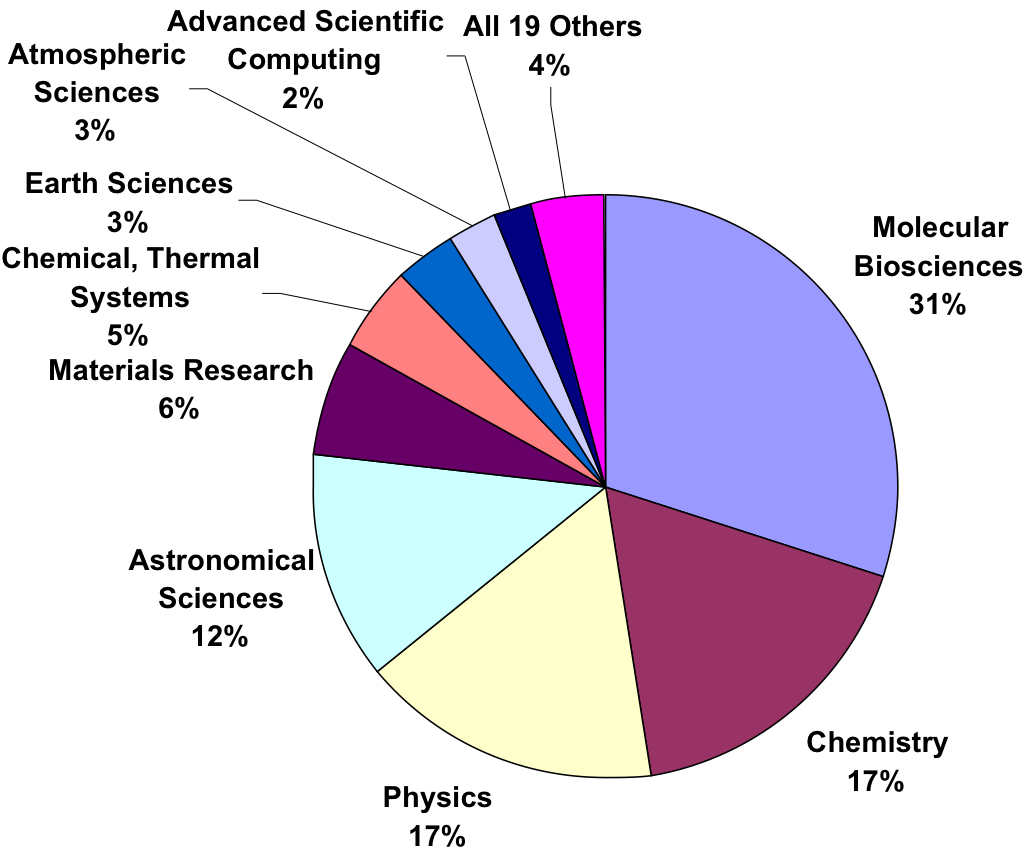
\includegraphics[scale=0.40]{figures/teragrid-discipline07}
\caption{\small 2007 Usage statistics for the TeraGrid.  (Reference
  \url{http://www.teragridforum.org/mediawiki/images/9/90/II_WorkShop_G-HPC_Nework_2009-Towns.pdf})}
  \label{tg2007}
\end{figure}


\begin{table}
 \small
\begin{tabular}{|c|c|c|c|c|c|} 
  \hline  Quarter & PIs & Current & Active & Allocations  & Usage\\
  & & Users  &  Users & (NUs) $\times 10^6$& (NUs) $\times 10^6$ \\ \hline
  Q3 2010 & 249 & 1,044 & 366 & 8,810   & 2,219  \\ \hline
  Q4 2010 & 254 & 1,040 & 356 & 11,720  & 2,658, \\ \hline
  Q1 2011 & 257 & 1,168 & 418 & 13,101  & 3,412\\ \hline 
\end{tabular} 
\caption{\jkimnote{need a caption for describing this table}}
 \label{} 
\end{table}



\subsection{Large scale life-science applications on the distributed HPC resources}
Traditionally, life-science applications have been regarded as non-HPC
applications.  Notably, only a few applications were actively pursued with
large scale computations.  Two representative examples are molecular
simulations and virtual docking calculations.  Interestingly, while
the former represents the case that the so-called scale up of bulk
synchronous techniques such as MPI is used as a main strategy to deal with
larger molecular systems, the latter represents the case that massive
independent tasks should be carried out, representing two different
application usage modes.

\begin{figure}
 \centering
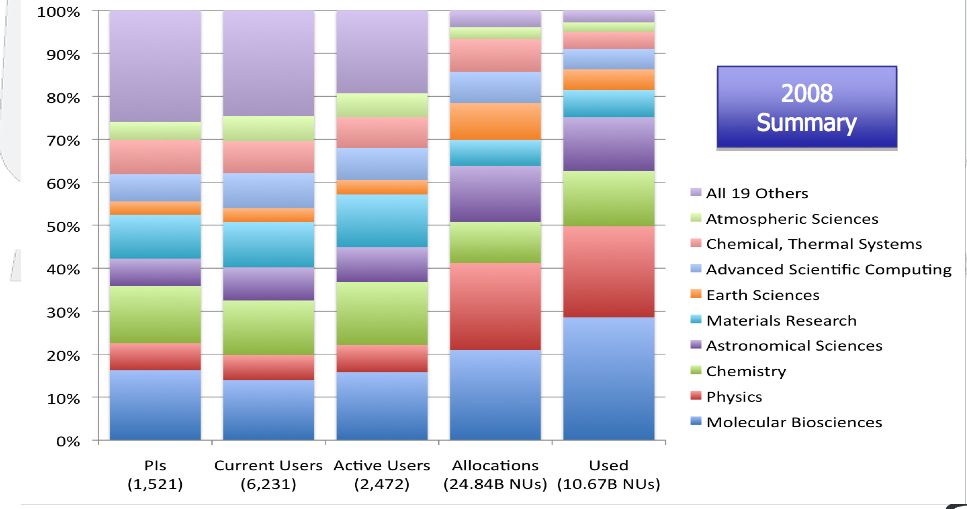
\includegraphics[scale=0.27]{figures/teragrid-discipline08}
\caption{\small 2008 Usage statistics for the TeraGrid (Reference
  \url{http://www.teragridforum.org/mediawiki/images/d/d8/DEISA-PRACE-May2009-Towns.pdf})}
  \label{tg2008}
\end{figure}

Meanwhile, the need of large-scale distributed parallel executions for
other life-science applications has grown due to the advances of
experimental techniques employing high-throughput approaches as well as
the advent of computing power and data management capacity.  For
example, Next-Generation DNA Sequencing (hereafter, NGS) technologies
challenge computational biology with unprecedented amounts of data
produced by their high-throughput capability.  Required data analytics
for processing such sequenced data along with dealing with genome data
sets available in public and private databases is overwhelmed by the
pace of growing data volume.  This poses the question on how the
challenge associated with the large volume data-management as well as the computational requirement
for analyzing large volumes of data are effectively managed.

Interestingly, the cyberinfrastructure considerations requried to
support a broad-range of analytical approaches and at the scales
required, has received less attention than the data-management problem
and algorithmic advances.  Thus not surprisingly, traditional
production cyberinfrastructure, such as the TeraGrid, have not been
used for such data-intensive analytics and distributed applications. There are multiple reasons,
but a couple of contributing factors are: (i) insufficient runtime
enviroments (and abstractions) to support concurrent computational
capabilties with large-data sets to support data-analytics (beyond
visualization) in an easy, scalable and extensible fashion, (ii)
insufficient support for user-customizable data-intensive "workflows"
that effectively hide the challenges of data-movement and efficient
data-management whilst managing concurrent distributed (computational)
resources.

Indeed, molecular simulations, virtual screening, and many other bioinformatics applications, particularly, regarded as the non-HPC applications could increase their usages dramatically by utilizing distributed scalable resources, which is, as presented in this work, addressed by a gateway development that implements a runtime environment for executions of target computation and distributed data management.

This work is predicated on three important trends: (i) the importance,
impact and percentage of TeraGrid/XD resources assigned to the
life sciences is increasing at a rate that is probably greater than
other disciplines, (ii) that gateways have proven to be a very
effective access mechanism to distributed HPC resources provided by
the TG/XD, and in particular a very successfull model for
shared/community access models, and (iii) that there are missing
capabilties and abstractions to enable the use of the collective
capacity of distributed cyberinfrastructure such as TG/XD, especially
those that can be used to develop gateways in an easy, extensible and
scalable fashion for both compute-intensive and data-intensive
applications. We introduce the DARE framework that is a SAGA-based
higher-level abstraction, and demonstrate its effectiveness as an
integral component of a wide-range of life-science gateways. We
use DARE as the underlying component for four different
gateways that use both TG/XD resources as well as LONI resources.


\subsection{Challenges in developing a gateway supporting distributed applications with heterogeneous multiple HPC resources}

Science Gateways, in particular, targeting the Teragrid community, have witnessed successful achievements in terms of the growth of the number of supporting researchers and computing time usages.  However, most of Gateways are not likely to consider a distributed application as a primary application usage mode.  Perhaps, a big reason is due to additional complexity to transform a target application to a distributed application.  Generally, the main developmental objectives for distributed applications are to achieve the key features such as interoperability, distributed scale-out, extensibility, adaptivity, simplicity-taken together referred as IDEAS.  Achieving such goals are, however, not trivial mainly due to the lack of tools for the coordination over multiple and distributed compute/data sites.  As we observe with the advent of federated grids such as Teragrid and its transition to eXtreme Digital (XD) environment, such requirements become harder to achieve as the number of connected sites grows as well as the computing power and the data storage capacity of each resource reach peta or exa scales.   More importantly, supporting a broad range of diverse execution patterns is critical considering different application usage modes for different life-science applications.  For example, in Table~\ref{table:four-applications}, application usages for four life-science applications focused on this work are summarized by contrasting conventional vs. distributed modes.  Last not the least, it is always challenging to respond effectively for upcoming demands of supporting new applications, distributed data management with new infrastructure, implementation of novel execution patterns, which is often eased by the development of a framework and its use for the efficiency in development cycle.   



\section{FOUR LIFE-SCIENCE APPLICATIONS}

\begin{table}
 \tiny
\begin{tabular}{|c|c|c|c|} 
  \hline Science  & Supported  & Conventional   & Example of  
  \\
  Domain & Appli- & Application & Distributed Application \\ 
  &  cation(s) & Usage Mode & Usage Mode \\  \hline \hline 
  
  Molecular   &  \texttt{NAMD} &  MPI-based  & ensemble-based   \\
   Dynamics  &  & single cluster execution & multiple (independent/ \\ 
   &  &  &  loosely-coupled)  \\ 
   &  &  &  execution \\ \hline
  RNA   & \texttt{SFOLD}, & single node   & multiple tasks with \\
  Folding   & \texttt{RNAFold} & serial execution &   distributed resources \\
  Prediction & &  & \\ \hline
  NGS data     &  \texttt{BFAST} & memory-intensive  & data-intensive\\ 
     analytics  &  &  single node execution   &  distributed resources \\ \hline
  Virtual  & \texttt{Autodock} &  many tasks   & many tasks \\
   Screening  &  & with a cluster  & with multiple resources \\
  (Docking) &  &  & \\ \hline

\hline
\end{tabular} \caption{Four life-science applications of interest and their usage modes.  Four gateways were developed for these applications using the DARE framework}
 \label{table:four-applications} 
\end{table}

Here we describe the four scientific applications briefly around the aspects primarily focused by the gateway development using the DARE framework

\textit{Large scale Molecular Dynamics simulations}

Over the past two decades, the field of biomolecular simulation has
exploded due to increases in computational power and parallel codes,
the emergence of accurate molecular mechanical potentials or force
fields and improvements in the methods~\cite{amber,mackerell2008,adcock2006}. A continually growing body of researchers apply atomistic and coarse-grained molecular dynamics (MD) simulation
methods to facilitate drug discovery, perform advanced materials
research, to design and understand biomolecular and designed
catalysts, and to provide fundamental insight into molecular
structure, dynamics and interactions\cite{meinke2009,mcdowell2006,beck2007,}. 

%Particular challenges include de
%novo protein and nucleic acid folding and structure prediction;
%correctly modeling induced-fit and conformational selection as drugs
%or other molecules interact with a target macromolecule; modeling
%large ensembles of biomolecules such as proteins in a membrane
%environment, viruses, and biomolecular machines such as the ribosome;
%combined quantum and molecular mechanical treatments for modeling
%chemistry; and improving conformational sampling and estimation of
%free energies and free energy pathways. 

In response to the perceived needs and importance of molecular
simulations, numerous high performance distributed memory parallel codes
have emerged in the past two decades (including NAMD, CHARMM, AMBER,
LAMMPS,GROMACS, etc.), and many now can
directly include quantum representations.  An interesting challenge in the MD community is, along with continuing efforts that tackle more scalable molecular systems with longer time trajectories using more powerful machines, to develop ensemble-based simulations over multiple HPC resources.  

\textit{NGS-driven genome data analytics}
In the past several years, there has been a major paradigm shift in biological/biomedical researches with the Next-Generation DNA Sequencing technologies\cite{mardis2008-tig,metzker2010,mardis2008-arghg}.  Their novel capabilities of cost-effective resequencing, full-scale quantitative transcriptomics, and holistic approach for cell development and cell differentiation using protocols such as RNA-seq. and ChIP-seq opens a completely new era for life-science researches\cite{sorek2010,mortazavi2008}.  In spite of such great opportunities, current NGS platforms challenges data analytics to deal with the sequencing data and the following bioinformatics analysis and inference.  For example, at this moment, NGS platforms produce typically billions of reads that comprise a short sequence mostly less than 100 base pairs with most of real experimental setting\cite{alex2009,trapnell2009}.  Furthermore, the increasingly effective cost-down trend causes the difficulty in management of significant size of data produced or related data sets that should be analyzed together.  
Generally, bioinformatics tools or applications developed for NGS data analytics are numerous and there is no sign to see the end of influx of new tools considering continuous innovations in the technologies and algorithmic advances in such tools.  In particular, we focus on the  important analysis of NGS data, mapping of NGS data reads on a reference genome.  It is noted that this analysis step should be applied first to proceed the following analyses targets more specific research goals such as genome variation, genome-wide association, comparative genomics, and other applications for investigating biological processes in a living cell.     

\textit{RNA structure prediction and beyond}
Defying the old biological dogma, positioning RNAs as a genome information intermediate between DNAs and proteins, during the last couple of decades, the number of scientific observations found that RNAs were involved significantly in gene expression and regulation\cite{joyce1999,cruz2009,encode2007,amaral2008}.  Now, with the well-known categories of non-coding RNAs such as miRNAs and riboswitches, in spite of their biogenesis that does not need to be translated into proteins, significant roles of RNAs are quite well recognized\cite{costa2009,ellington2007,baek2008,blouin2009,henkin2009}.  Importantly, RNA functions by forming required structure(s), and the pattern of structure formation of RNAs are somewhat contrasted to proteins that are mostly folded into highly specific 3-D structure\cite{roth2009}. For example, riboswitches chose one of two alternative structures, in response to meta-bolite binding, consequently resulting in two different gene regulation stages, i.e., turning on downstream gene synthesis or turning it off\cite{montange2008,dambach2009,weinberg2007}.  Therefore, RNA structure prediction has been the major area for RNA studies and may noticeable progresses were made recently for RNA 2D structure prediction as well as 3D structure modeling\cite{shapiro2007,mathews2006,ding2003}.   

\textit{Drug Discovery via Virtual Screening strategies}
For small molecule drug discovery, virtual screening using a docking method has been widely utilized and an immediate requirement for massive docking calculations against a chemical database has been attempted by managing such many tasks using a local cluster, HPC cluster, grids, and clouds\cite{levesque2009,yim2010}.  The nature of required application usage mode for virtual screening methods is a generic example of many task computing, implying that pleasingly parallel massive tasks carrying out a docking computation should be executed.  In spite of such well-established protocol, the challenges in drug discovery finding putative inhibitors for target receptors are not resolved due to intrinsic difficulties with underlying physico-chemical models associated with the issues with scoring function, receptor flexibility, and docking strategy itself\cite{amaro2010}.  Therefore, more computing power and scaled calculations by varying the parameters for virtual screening are needed in order to understand the accuracy of results, suggesting the need of scalable infrastructure is highly appreciated while the application usage mode is generally intact.   

\subsection{Computational requirements and challenges}

A growing limitation of applications in the life sciences is that workflow, data management, and
analysis have become rate limiting steps: what is missing is support for the end-to-end execution requirement of applications.

We also need to move to tiered sets of computational resources.  For
example, one can imagine running large ensembles of MD engines on
tightly coupled parallel machines (like Ranger or Kraken) with
real-time data streamed to separately running analysis and
visualization resources (Lonestar, Spur), with on-the-fly monitoring
to analyze convergence, interesting phenomena or problems.  This also
provides the means for possible steering, for example by spawning or
stopping separate elements of the ensemble to sample more or less in a
particular region of interest.  In addition to real time monitoring,
hidden correlations in the data require the saving of coarser grained
simulation data on longer term (1-2 year) disk resources for further
analysis and mining using less tightly coupled computational
resources, and ultimately placing reduced and derived data sets
seamlessly back to the campuses, archivers, and for public
distribution.  Not only does this support the need for diverse sets of
computational resources, large-scale storage and data transfer
requirements for sophisticated analysis and visualization, and
high-bandwidth networking, it also drives the need for software tools
that facilitate the complicated workflow management, that allow
dynamic monitoring, starting and stopping of ensemble elements without
losing access to the global communications fabric and local
connections, and that provide the means for facilitating data
management and analysis.

In essence, the move from executing an individual task to \textit{large
  ensembles} of coupled/loosely/uncoupled tasks requires scientists to spend
significant time on compute and data management problems, instead of
core science.  The quantitative shift (massive distributed parallel
compute and data resources) implies qualitative change in the way how life-science applications are being served for scientific discovery. 

\jhanote{At the end we propose DARE based Gateways as a solution}


\section{DISTRIBUTED ADAPTIVE RUNTIME ENVIRONMENT}
In order to provide a means for end users to utilize a scientific application with scalable heterogeneous distributed computing resources, we develop the Distributed Adaptive Runtime Environment (DARE) framework\cite{dareurl}.  As shown in Fig.~\ref{fig:dare-arch}, the framework comprises, basically, three layers, the Access Layer, the Services Layer, and the Resource/Provisioning Layer, whose underlying development mechanisms are independent and modular but unified under the framework.  The core layers of the DARE framework, the Services Layer and the Resource/Provisioning Layer are powered by SAGA and SAGA-based Pilot-Job abstraction, SAGA-BigJob\cite{saga-ccgrid10,saga-royalsoc,saga-web,jha2009developing,ecmls10, ecmls11}, and collectively constitute a runtime environment for distributed applications.  The Access Layer is built upon the open source web application framework, pylons\cite{pylonsurl}.  The combination of the open source web application technology and the runtime environment carrying out a distributed application management system is the main design strategy of the DARE framework for the development of a lightweight, extensible, full-fledged distributed computing science gateway quickly and effectively\cite{pylonsurl}. 

\subsection{SAGA and SAGA-BigJob abstraction}
SAGA is an API providing the basic functionality for developing distributed applications, tools and frameworks\cite{saga-web}. The key advantages of the development using SAGA include i) to provide a general-purpose common functionality while hiding complexity of heterogeneity of back-end resources ii) to provide building blocks for constructing higher-level functionality and abstractions iii) to provide the means for developing broad range of distributed applications such as gateways, workflows, application management systems, and runtime environments.   Interestingly, SAGA provides a simple way to support python scripting for building distributed applications via python-binding.  SAGA-BigJob was introduced for a pilot-job abstraction with which various execution patterns and application usage modes are implemented.  Previously, we demonstrated how SAGA-BigJob was able to execute scientific applications categorized as pleasingly parallel applications and loosely coupled applications in scalable distributed resources\cite{saga-royalsoc,jha2009developing, ecmls10, ecmls11}

With the framework built upon SAGA and SAGA-BigJob, the fundamental design objectives of Interoperability across different infrastructure, Distributed Scale-Out, Extensibility, Adaptivity whilst preserving Simplicity (IDEAS), which constitutes essential requirement for distributed applications, are achieved in a remarkably effective way.



\subsection{Architecture : The Three Layers -- Access Layer, Services Layer and Resource /Provisioning Layer}

\begin{figure}
 \centering
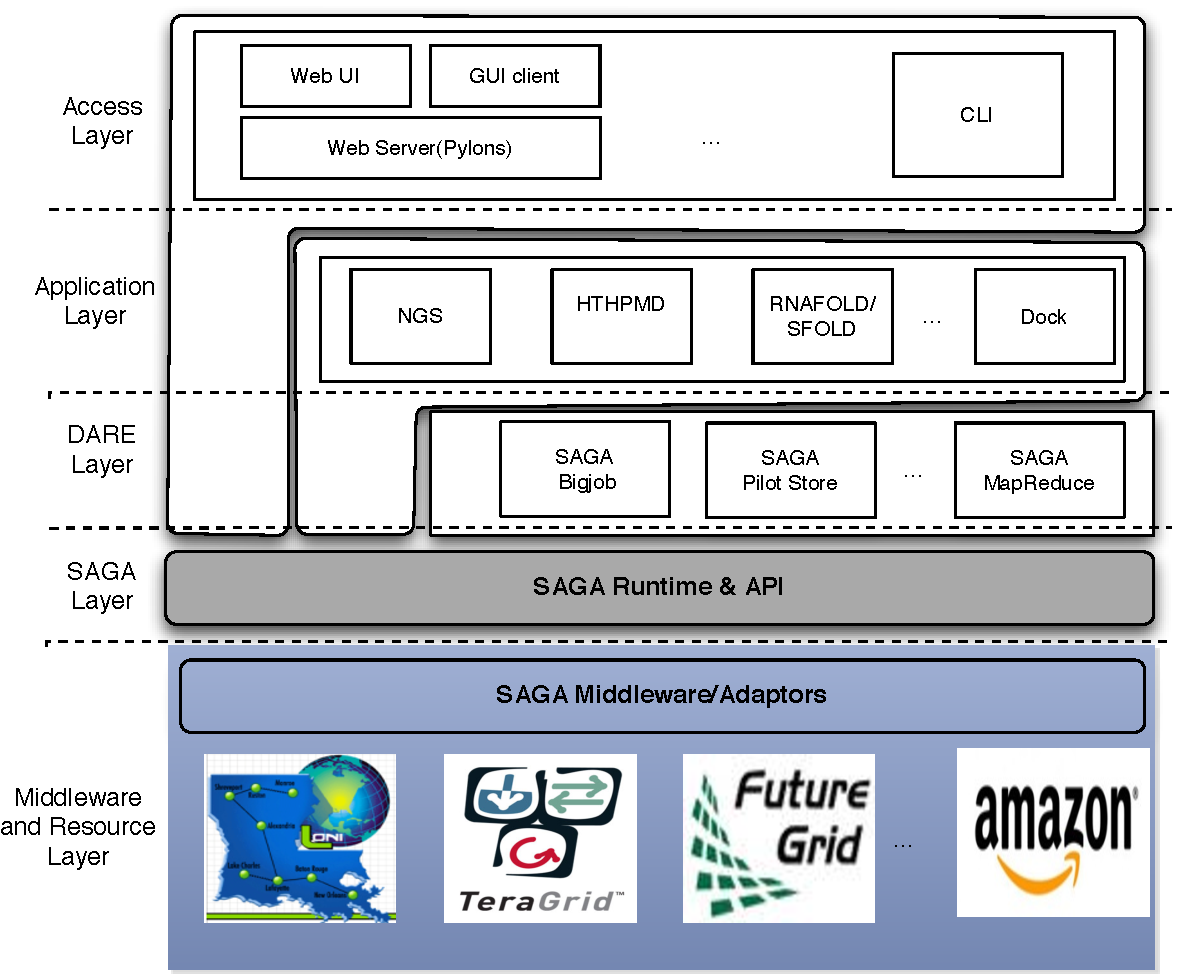
\includegraphics[scale=0.40]{figures/DAREOutline.pdf}

\caption{\small Dare architecture.}
  \label{fig:dare-arch} 
\end{figure}

 

%Level 2: (i) Computational aspect, (ii) Data management and movement, 
%
%Level 1: (iii)providing user interface


\textit{Access Layer}  The Access Layer is composed of a web server and User Interface (UI).  UI mediates the interactions between a user and a web server, and is primarily important for enhancing user experience.  Depending upon types of UI, three-tier or two-tier gateway structures are possible.  For example, if the web server is accessed via web pages or a remote client, the overall architecture is regarded as a three-tier architecture in which a user desktop, a server, and back end resources are independent to each other and their connection is under control by the DARE framework.  Currently, the framework employs the use of web UI as a primary means for a user access.  On the other hand, if Command Line Interface (CLI) is preferred, the overall architecture becomes two-tier due to no need for the existence of a remote user system.  

The Model-View-Controller (MVC) architecture model that underlies the pylons web application framework is very effective and advantageous in many ways for the Access Layer. For example, database creation, management, and transaction are extremely simple and robust to facilitate authentication steps and job/data creation and management by storing or retrieving related data.  Additionally, UI creation/development and the connection between server-side services (provided by the Services Layer) and UI-based user interactions are also surprisingly simpler compared to other existing approaches, requiring less programming efforts.  For example, it is well appreciated that for a science gateway development, the utilization of databases and server-side programming are non-trivial tasks.         

\textit{Services Layer}
This layer is composed of three sub-layers such as the application layer, the DARE layer, and the SAGA layer.  The application layer is the only layer requiring a developer to build their own.  Since target scientific applications differ in optimal application usage modes along with favorable execution patterns with different distributed resource characteristics, it is a developer's responsibility to find a better science logics, which is non-trivial if distributed resources and distributed data management are needed.  Indeed, SAGA and SAGA-BigJob mitigate such demanding efforts imposed to a developer with simple but powerful ways.  For example, by varying SAGA-BigJob configuration with a minimal effort, optimized execution usages of target computations for pleasingly parallel, loosely coupled, and strongly coupled applications, are quickly implemented.  As presented in this work with four different gateways for four different life-science applications, once figuring out preferable application usage modes as well as parallelization strategies, a gateway developer easily constructs an optimized runtime environment for a target application with distributed resources in a relatively short development cycle.   


%The web interface will be connected to remote job submission via a job scheduling and monitoring thread. This thread starts with pylons application and continuously communicates with local database server to find new jobs and it also acts as a scheduler for new jobs. Once this thread finds a new jobs it will start preparing the configuration files for that particular job from the user and afterwords it will start the remote job submission via application specific SAGA-Bigjob.

Importantly, data movement should be carefully considered for the Services Layer is built because the movement of data sets such as input, output, temporary files becomes a major challenge, as we have shown recently, in the case of data-intensive application\cite{ecmls11}. At this moment, GridFTP is used as a primary protocol for data transfer, and Table~\ref{table:NGS-Distributed-file} highlights the significance of data transfer with data analytics for DARE-NGS with a model system, human genome.  It is noted that in SAGA level, the emerging programming model for distributed data management such as MapReduce and cloud utilization are already supported\cite{abstractions-azure,saga-ccgrid10}.

%
%All the above components are well connected but loosely coupled from each others as well so this provides the development of different kinds applications very simple and fast.

\textit{Resource/Provision Layer}
The utilization of distributed heterogeneous resources is critical for a science gateway.  Most of gateways relies on the approaches in which multiple resource utilization is limited, presumably, for pleasingly parallel multiple tasks.  Owing to SAGA and SAGA-BigJob, interoperability, distributed scale-out, and adaptivity are fully supported for distributed applications.  In particularly, various SAGA adaptors contribute to achieve interoperability for inter-HPC-grids, HPC-cloud, and other hybrid resources.  In SAGA web site (http://saga.cct.lsu.edu), useful information including how to develop a new adaptor can be found.  On the other hand, SAGA-BigJob has been shown for its capability for various adaptive execution supports in the cases of Replica Exchange Molecular Dynamics, hybrid CFD-MD, and NGS data analytics\cite{saga-royalsoc,coupled,ecmls11}.    


The access layer is connected to service layer with the help of configuration files. The job-scheduling/monitoring thread  which starts along with the web server is responsible for writing the job configuration file which changes for every single job. Apart from this job configuration file there are two other configuration files, first one has the resource list which is common for any application  (DARE-NGS, DARE-HTHP etc. ) and the other one is application specific configuration on each resource containing the paths for executables, input, output directories. once the job-scheduling/monitoring thread creates the job specific configuration file, it invokes another thread which starts reading the configuration files assigned to it and acts as a manager for this particular job. And this thread is responsible for transferring the appropriate input files to different resources, submitting and running the required jobs requested by user and getting back the output files which are inturn zipped and provided to user for download via web. But , we have keep in mind the uploading input files and downloading output file via web browser has not been implemented since the files sizes are too big to handle via browser and we are working on finding ways to handle this kind of situation. SAGA plays an important role with this job manager thread which makes the remote job submission and files/folders movement across different machines very simple and easily usable.

 \begin{table}
\small
 \begin{tabular}{|c|c|c|c|c|} 
 \hline 
Genome & Index           & Resource    & \# of Cores             &	TTC  \\
  Type               &  File      & & (\# of nodes & (sec)\\  
  & Size (GB)  &   & or VMs) & \\   \hline
 B. Glumae &0.435& R&	64(4)	&1067 \\
\hline                  
B. Glumae &0.435& QB	&	64(8)	&719 \\
\hline
 B. Glumae &0.435&R/QB	&	32(2)/32(4) &919 \\
\hline
 B. Glumae &0.435& FG &	64(8)	&712 \\
\hline
 B. Glumae &0.435 &  R/QB/FG &	24(2)/24(3)/& 1022\\
& &  & 24(3) & \\  \hline  \hline

HG18-Chr21 &1.9& R	&	64(4)&1145 \\
\hline
HG18-Chr21 &1.9& QB	&	64(8)	&924 \\
\hline
HG18-Chr21 &1.9& R,QB	&	32(4)/32(2)	&1170 \\
%\hline
%HG18-Chr21 &1.9& FG	&	64	& \\
%\hline
%HG18-Chr21 &1.9& R/QB/FG	&	24(2),24(3),	& \\
%&& 	 &24(3)&\\
\hline
\hline
HG18 &127& R	&	256	&9586\\
\hline
HG18 &127& QB	&	256	&919 \\
\hline
HG18 &127& R,QB	&	128(16)/&7582 \\
&  &  &   128(8)  &  \\
\hline
\end{tabular}
\caption{Comparison of Time to Completion (TTC) required for the NGS data mapping calculations using BFAST (match step).  Three genome types, HG18, HG18-Chr21, B. Glumae represent a human genome, chromosome 21 of HG18, and the genome of a microbe Buerkerholderia Glumae.  Three compute resources are Ranger (R), QueenBee (QB), and FutureGrid Cloud (FG), respectively.  The number of tasks for carrying out the required mapping calculation is 30 for B. Glumae and 32 for HG18 and HG18-Chr21.}

  \label{table:NGS-Distributed} 
\end{table}




 \begin{table}
 \small
 \begin{tabular}{|c|c|c|c|c|c|c|c|c|} 
 \hline 
	                      &  Index File	&Raw &	Processed\\
	                      &&Short Reads& Short Reads\\
\hline 
Size  (GB)    	             &127&	9	&3.81\\
 \hline                       
LW to QB (s)   & 1814.29&	128.57&  NA\\
  \hline
LW to Ranger & 21166.67 & NA & NA\\
   \hline
LW to QB(s)    & 7105.67& NA &NA\\
 \& QB to Ranger(s)     &&&\\
 \hline
QB to Ranger(s)   	&NA&NA& 158.33\\
\hline
Min Total time(s)    &	7105 &	128&	158.33\\
 \hline
\end{tabular}
\caption{File transfer time with GridFTP between a local workstation (LW), QueenBee (QB), and Ranger with the case of Human Genome Exome data.  }

 \label{table:NGS-Distributed-file} 
\end{table}


\section{FOUR DARE-BASED GATEWAYS}
\subsection{DARE-NGS}
Our DARE-NGS gateway (http://cyder.cct.lsu.edu/dare-ngs) supports Genome-wide analysis on Teragrid and provides currently the mapping process using BFAST that aligns the large number of short reads sequenced from NGS machines onto a reference genome sequence, which is the first step in scientific discovery utilizing NGS sequencing-based protocols such as the whole genome resequencing, RNA-seq, and ChIP-seq.  De novo assembly without reference genome information is still in early stages.  Note that due to its design strategy, including other analysis tool such as assembly or extending to a pipeline with other tools successively applied after the mapping with DARE-NGS are straightforward and underway at this moment.

It is worth mentioning that the computational complexity
of the analysis (e.g. mapping) depends, upon other things, the size
and complexity of the reference genome and the data-size of short reads.
Given that these can vary significantly, the computational
requirements of NGS-analytics also varies (even between data-sets of
similar size).  Thus an efficient, scalable and extensible analytical
approaches must be supported by any framework supporting
NGS-analytics.  The current service provided by DARE-NGS focuses mainly on the mapping step among bioinformatics tools with BFAST for single end NGS data or BFAST+BWA for paired-end data, and eventually supports a pipeline including genome variation studies for finding SNPs and small Indels.

Recently, we reported our exploration of NGS analytics using DARE-NGS with the HPC grid such as TeraGrid and
Cloud environment of FutureGrid\cite{ecmls11}. 



\begin{figure}
 \centering
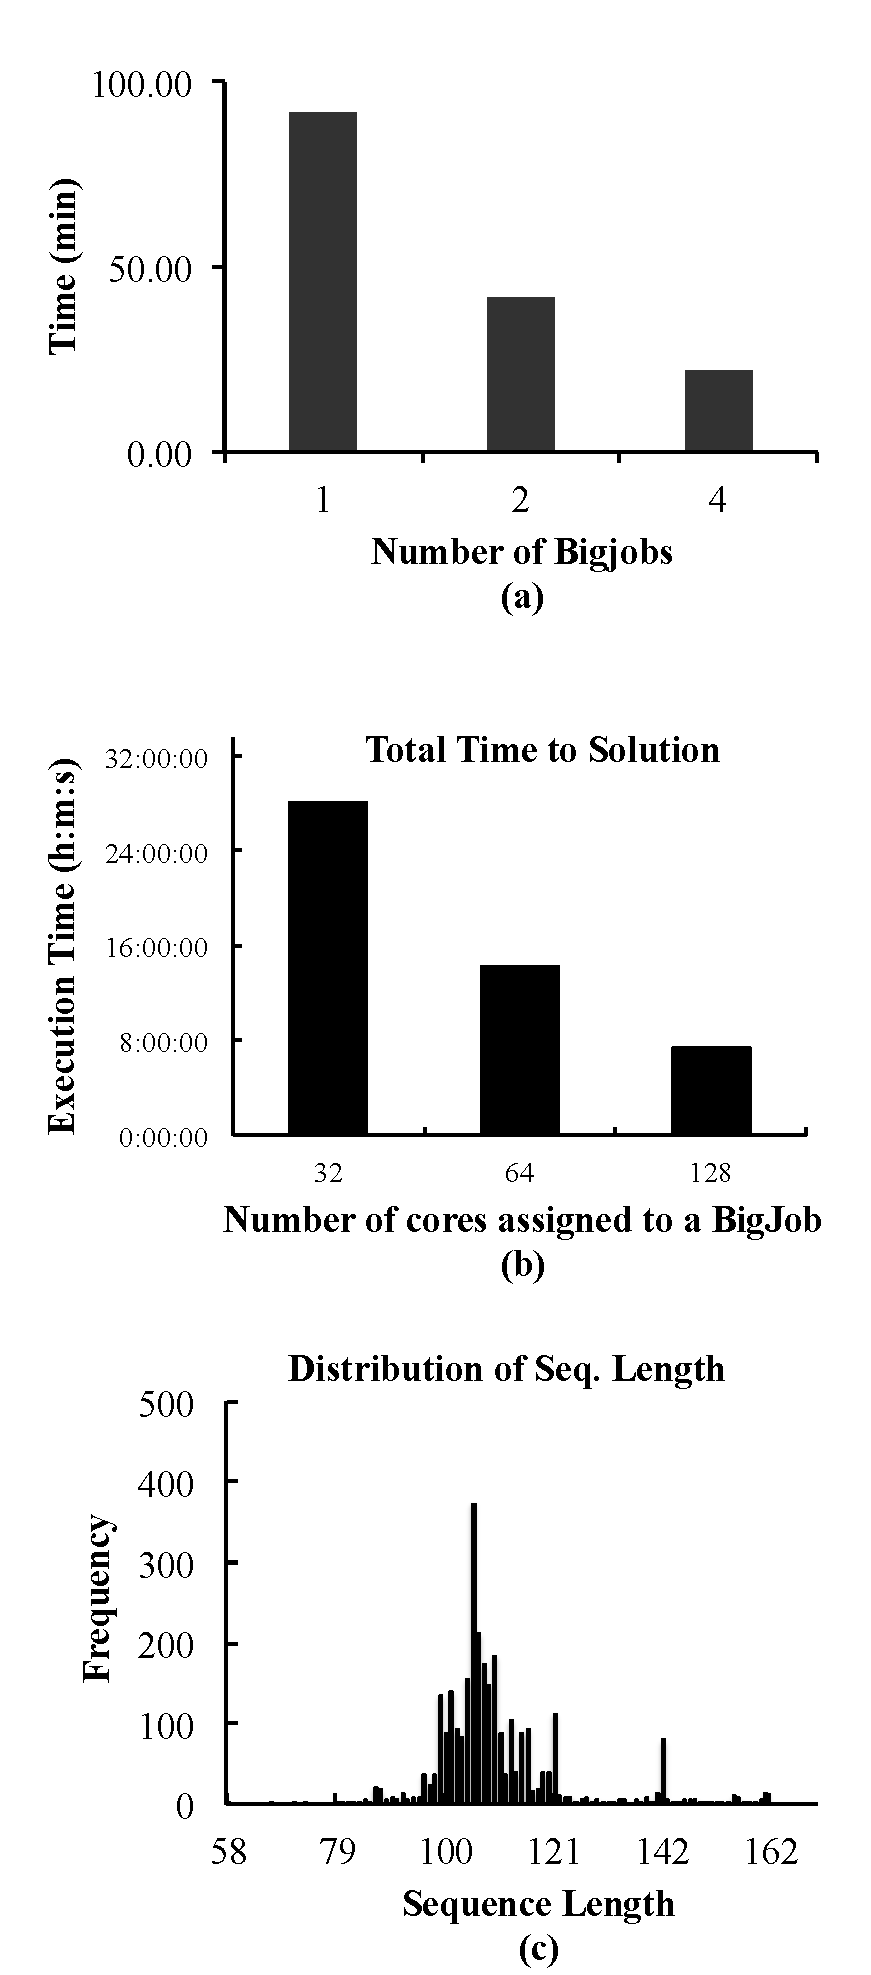
\includegraphics[scale=0.40]{figures/dare-rfold-result.pdf}
\caption{\small Massive concurrent calculation capability is presented with the results obtained with DARE-RFOLD. The total 2910 SAM-I riboswitch sequences are injected into the DARE-RFOLD for sampling of Boltzman-weighted secondary structures.  SAGA-BigJob handles these many tasks by decoupling the resource assignment and execution of each task, collectively allowing an efficient management of many tasks. In (a) and (b), time-to-solutions with different configurations of BigJob are compared in terms of the number of BigJobs (a) and the size of a BigJob (b).  In (c), the distribution of sizes of 2910 input sequences is illustrated.  This distribution is directly associated with the distribution of time-to-solutions of all 2910 tasks.}
  \label{fig:dare-rfold-result} 
\end{figure}

As shown in Table~{NGS-Distributed} presenting the comparison of various execution scenarios with multiple resources including a cloud system, DARE-NGS was successfully developed with HPC grids and a cloud environment.  Our initial attempt, however, indicated several issues with an emerging distributed environment.  For example,  we observed that the large data management in FutureGrid cloud demanded to us Walrus data storage system, but an access by multiple VM's failed often.  This situation should be managed appropriately since our case with human genome mapping needs the disk space more than the default disk space of the current cloud environment.

For the data-intensive computation such as NGS analytics, file transfer processes are important for the total time-to-completion, and Table~{table:NGS-Distributed-file} hints such issues.  At this moment, our four gateways employs GridFTP as a default protocol.



\subsection{DARE-Rfold}
To support nc-RNA research and broadly for the community who is interested in the utilization of RNA structure prediction for their research goals and education purposes, we have been developing a gateway, DARE-RFOLD, with which a user is able to predict the Minimum Free Energy (MFE) secondary structure or an ensemble of structure sampled with a Boltzmann-weighted sampling scheme.  

Notably, many challenges in the computational investigation of RNA folding dynamics exist.  For example, the support of high-throughput of highly-parallel tasks on heterogeneous distributed resources is critical.
We demonstrated the use of DARE-RFOLD for the exploration of RNA folding energy landscape and structural characterization of SAM-I riboswitch sequences, which was greatly facilitated by the flexibility of our DARE framework and the capacity for many task computing to deal with 1000 structures from each sequence among 2910 sequences of SAM-I RAN family\cite{ecmls10}. 


\subsection{DARE-DOCK}
DARE-DOCK was developed to support the basic virtual screening and the target application is Autodock\cite{autodock}.  Autodock-vina is provided as a main tool to utilize its support for fine-grain parallelism with multi-threading multi-core support, whose capability is thus considerably enhanced with task level concurrency implemented with pre-processing that breaks the set of ligands in a given chemical database into many sets\cite{autodock-vina}.  

%\begin{figure}
% \centering
%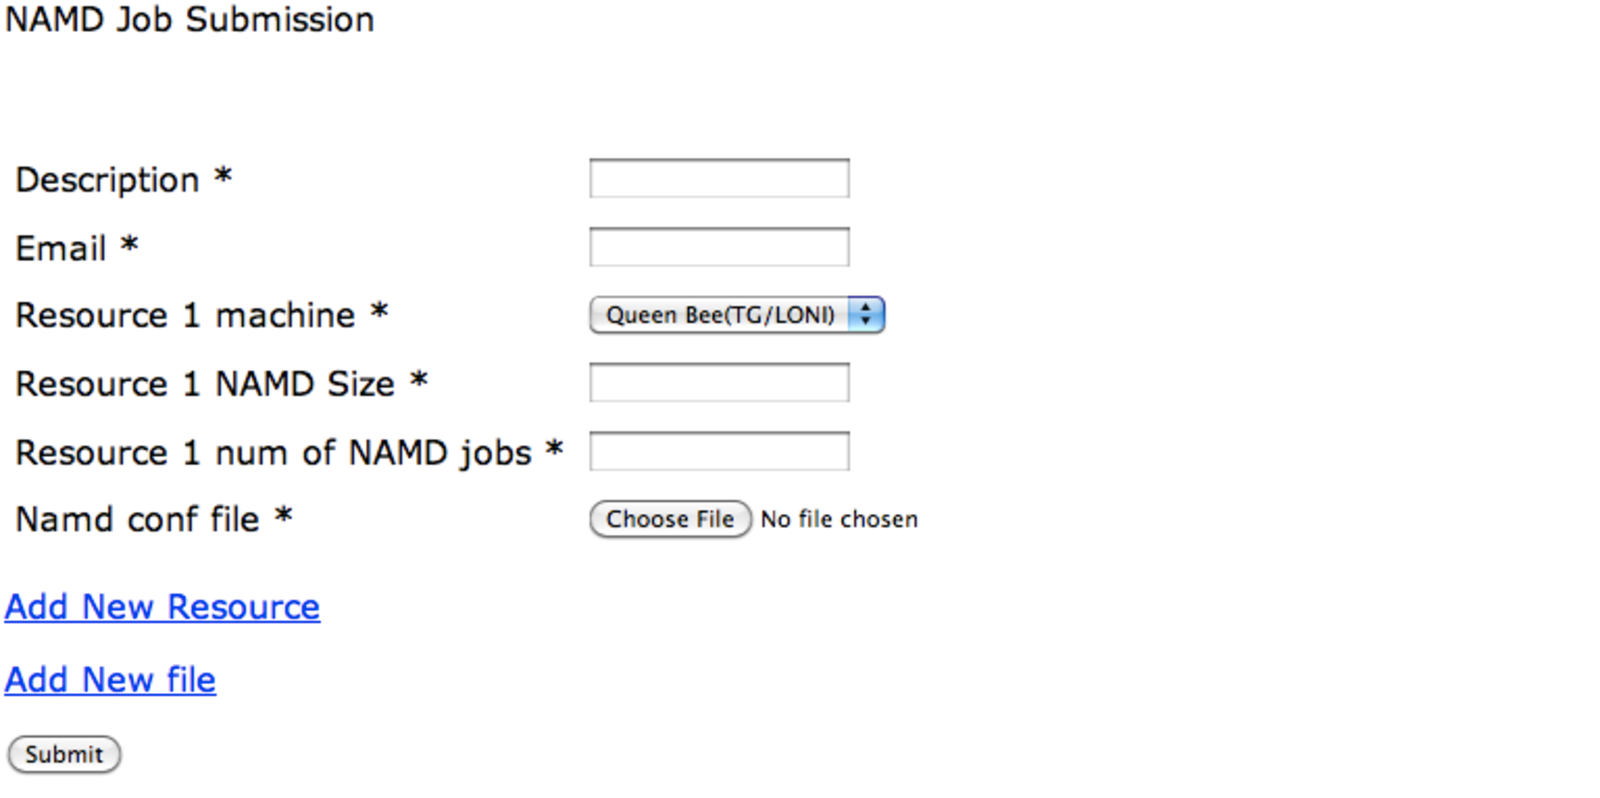
\includegraphics[scale=0.35]{figures/NAMD1.pdf}
%
%\caption{\small NAMD job submission web page form through DARE-HTHP} 
%\end{figure}

\subsection{DARE-HTHP}

An important challenge in modern biomolecular simulations, that has
received insufficient attention is not to get single long-running job
completed, but managing and executing multiple instances of the same
(or similar) physical system.  There are multiple reasons behind this
-- ranging from higher accuracy to reduced time-to-solution. For
example, multiple ensemble-member runs of the same physical system
enable better sampling In some cases, such as free-energy
calculations, multiple ensembles of the same system need to be
utilized. And even where a single long-running simulation is required,
thanks to algorithmic advances, such problems can be transformed into
the more {\it tractable} problem of solving multiple shorter run
simulations.



A ensemble simulation framework is required which has the following
characteristics: (i) Usable on a range of underlying distributed
resources and independent of the machine/resource-specific middleware
and services (i.e. scale-across), (ii) Efficiently manage both
scale-up and scale-out of ensembles -- possibly scaling upto
tens-of-thousands, if not millions of ensembles, with varying degrees
of coupling, (iii) Effective for a range of physical model sizes --
from thousands of atoms to hundreds of thousands of atoms, (iv) All of
the above without being tied to a specific underlying MD kernel, (v)
Extensible and Interoperable with emerging computational platforms such
as clouds.


When the user submits the from to run on Futuregrid cloud environment these files are also transferred to  different VM's 
 and jobs are also launched according the job configuration provided by user. To provide this provision for users we have prepared images which have SAGA and 
other required adaptors installed along with NAMD and MPI as well.  These images are used to launch multiple VM's and job submission similar to grid environment.

 \begin{table}
\small
 \begin{tabular}{|c|c|c|c|c|} 
 \hline 
 Number           & Resource    & \# of Cores             &	TTC  \\
of tasks                &     & (\# of nodes           & (sec) \\  
  &   & or VMs) & \\   \hline
8& R&	64(4)	&141\\
\hline                  
8& QB	&	64(8)	&176 \\
\hline
4/4&R/QB	&	32(2)/32(4) &151\\
\hline
8&FG	&	64(8) &414 \\
\hline
2/3/3&R/QB/FG	&32(2)/24(3)/24(3)	 &384\\
\hline


\end{tabular}
\caption{8 tasks of NAMD run over different resources, Three compute resources are Ranger (R), QueenBee (QB), and FutureGrid Cloud (FG), respectively.}

  \label{table:HTHP-Distributed} 
\end{table}


\begin{figure}
 \centering
 \fbox{

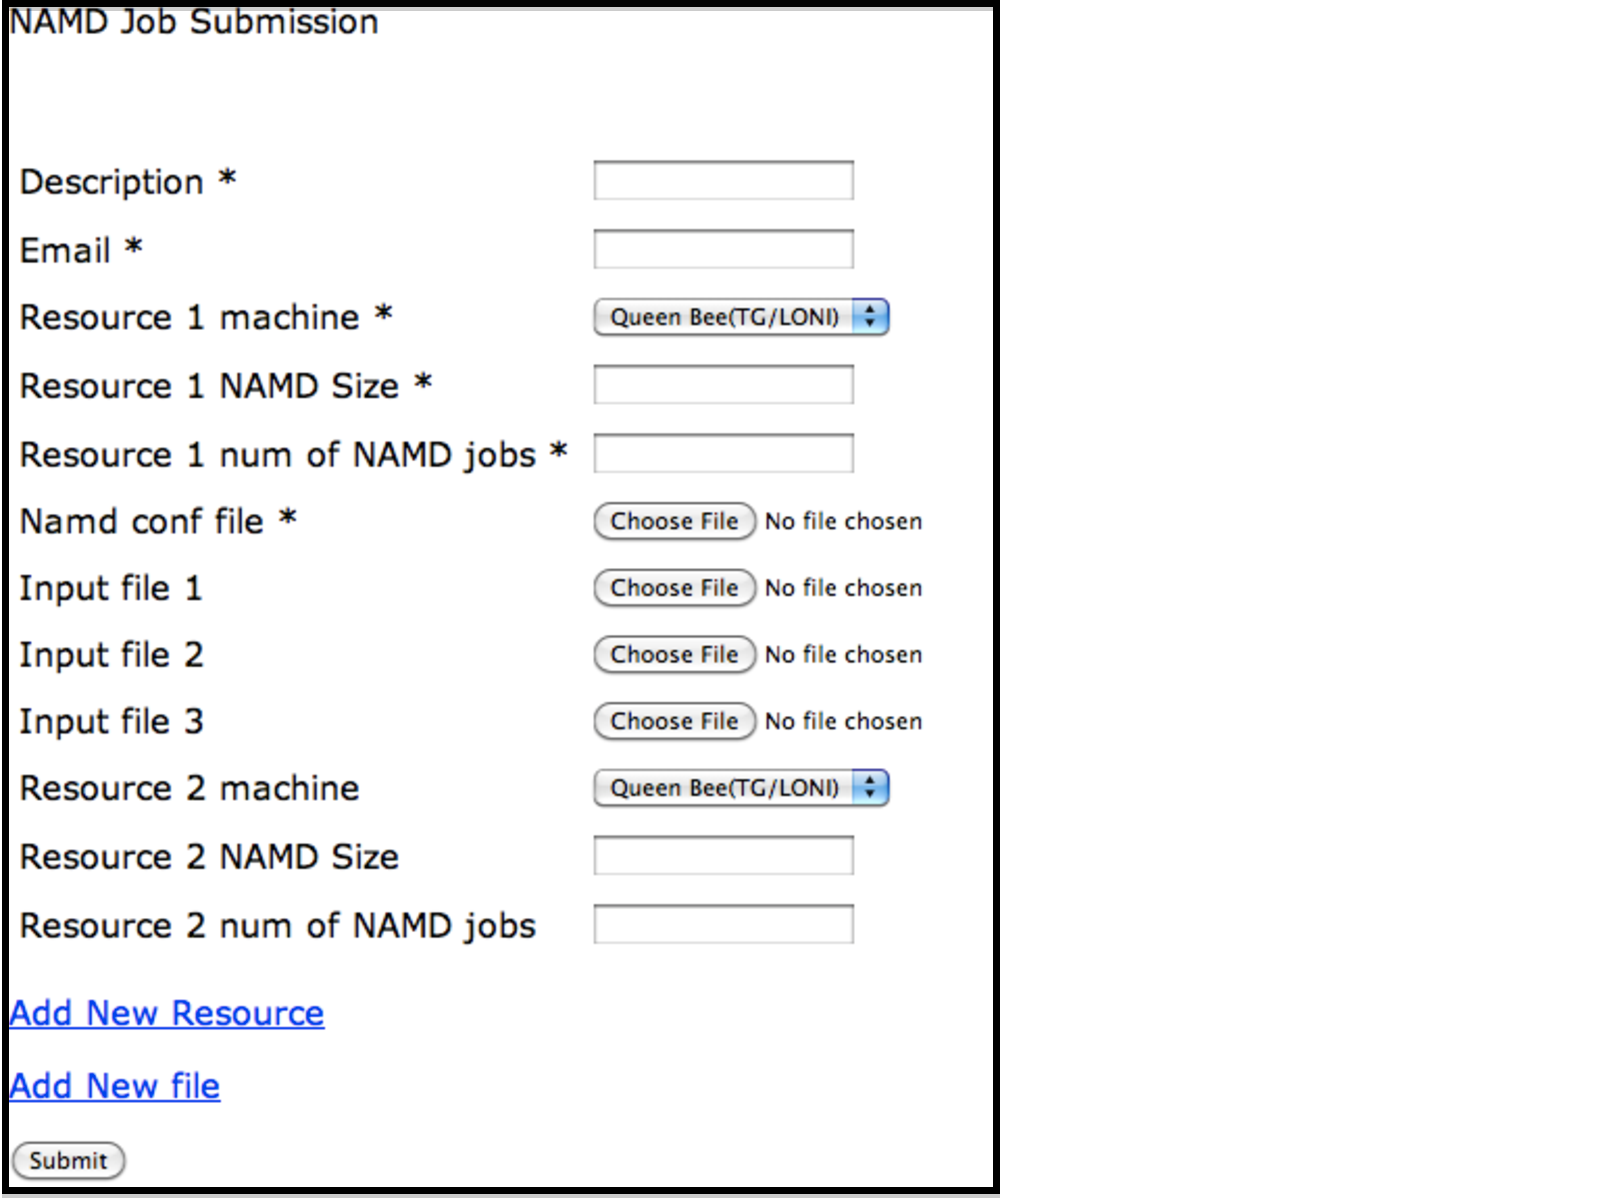
\includegraphics[scale=0.35]{figures/NAMD2.pdf}
   
  }
\caption{\small NAMD job submission web page form through DARE-HTHP. Here, the form indicates the usage mode with multiple resources.  The simple case with a single resource is default, and a user can expands the form by adding more resources as shown.}
  \label{fig:NAMD2}
\end{figure}


\section{Concluding Remakrs}

\textit{Achieving IDEAS : Interoperability, Distributed
  scaled-out, Extensibility, Adaptivity, and Simplicity}

%\smnote{ 1) Lets say we have "n" read files and with DARE it takes
%  around time "t" time for matching step if we run it serially it
%  would take n*t time. It probably exceeds wall time limit. Therefore
%  speed up in match step depends how many number of read files we
%  generate and process concurrently.  2) Yes we were able to process
%  the complete run with entire Human Genome on QB and Ranger
%  separately. (**I am currently working this to utilizing QB and
%  Ranger together.)  4) it should clearly provide the advantage with
%  multiple resources. If we want to use the cloud resources from India
%  to complete Human Genome run it is not practically possible because
%  of the current limited disk size access provided by the FG
%  Eucalyptus resources. Because whole human genome index files are of
%  size 129 GB for Bfast matching step as opposed to HG 18 Chromosome
%  21 with size of 2 GB index files. On the other hand it also requires
%  the temporary files disk space.  Thus it is important to utilize
%  large capacity resources like QB and Ranger divide the work load
%  across machines.}  
  
  
  Here, we present how the objectives of IDEAS are
accomplished with the DARE gateway examples.  First of all, the theme
of Simplicity is considered from the underlying SAGA-based API,
through a Pilot-Job abstraction, SAGA-BigJob, and the design of the
DARE architecture.  All of components in the DARE framework are
independent to each other due to its modular structure.  Additionally,
the framework provides the key functionality for job management and
data management with heterogeneous distributed resources in a flexible
mechanism to support various execution patterns and application usage
modes as well as the full-fledge access layer with the web server
framework.  Along with this backbone template, a developer can quickly
implement his/her own scientific logics in the application layer with
python scripts.  Secondly, the theme of Distributed scaled-out might
be illustrated with Table~\ref{table:NGS-Distributed}.  Here, two
large TeraGrid systems, QB and Ranger, were used for the match step in
BFAST pipeline.  It is noticeable that we compare different usage
modes, for example, using one resource or two resource altogether with
the same configuration for the computation.  As we demonstrated in
numerous publications, having more resources and using those scaled
computing power benefits to decrease the time-to-completion.  The
results of the cases in Table~\ref{table:NGS-Distributed} indicate
also there are interesting aspects due to the complexity of scientific
applications.  For example, in the NGS data alignment using BFAST, we
should consider the optimal condition with the task level concurrency
considering how the reference genome indexes are utilized for chucks
of short read data\cite{ecmls11}.  Extensibility is an important theme
in our DARE-based gateway development, and indeed, many levels of
extensibility are easily utilized.  While SAGA itself provide the
capabilities to expand its lineup with various adaptors to deal with
emerging new environment such as clouds, SAGA and SAGA-BigJob,
combined together, provides great flexibility to extend scientific
capability of a gateway. For example, with DARE-RFOLD, we attempted to
make a pipeline for another capability beyond RNA secondary structure
prediction.  We demonstrated recently the output from the RNA
secondary structure prediction could be utilized for Riboswitch gene
annotation with structural information.  Furthermore, with the open
source pylons framework, incorporation of many web technologies is
achieved efficiently.  Interoperability is what SAGA-based approaches
enjoys in a full scale with numerous adaptors as well as support of
programming models such as MapReduce.  Finally, Adaptivity is
importantly dealt with in the design of the DARE framework.
SAGA-BigJob has many advantages to be agile to change the application
usage mode from one to the other.  In
Fig.~\ref{fig:dare-rfold-result}, the result compares with two
different configurations of BigJob size, for example.  Note that not
only varying the size of a BigJob, other possible usage modes
supporting a case of loosely coupled applications and a case of
dynamically changing parallel/concurrent configurations in the
fine-grain parallelization (for example, MPI configuration) as well as
the coarse-grain parallelization are effectively designed.
In summary, with the DARE framework, the development of a science gateway that supports distributed applications including novel data-intensive life-science applications and that utilizes emerging distributed computing/data resources such as TeraGrid/XD and cloud environment contributes the advances of life sciences.    


\section{Acknowledgments}




\bibliographystyle{abbrv}
\bibliography{tg11}




\end{document}

